\documentclass{article}
\usepackage{graphicx} % Required for inserting images
\usepackage{tikz}
\usepackage{tkz-euclide}

% same question but before you do the square calculation apply changes where ranges of numbers map to other ranges of numbers

\begin{document}
\section{Pipeline Parallelograms}
Coastal Gaslink, a gas company, is planning out their latest Liquified Natural Gas Pipeline and needs to verify the validity of the plans. The scientists back at the lab have noticed a drop in pressure around some sections of the project in their simulations, which they suspect is a square formed in the network. Because of their lousy recordkeeping and haphazard nature, the numbers have been smudged and cannot be read normally. As a result you have been provided a number of transformations to apply to the coordinates first, then a subsequent amount of lines which has two sets of two numbers separated by a comma. The first set of numbers is the starting coordinate range and the second set is the ending coordinate range, as an example 1 7, 8 14 means that 1 will translate to 8 and so on up until and including 7. Both the first number and the second number of each set is inclusive. After the transformations there will be an empty line. Next you will be given a number of vertices and then a list of X and Y coordinates that represent junctions in the pipeline. Negative numbers map the same as positive numbers. From this input you should output the original coordinates of all unique points that form squares.
\subsection{Example Input}
\begin{verbatim}
    3
    1 7 8 14
    20 26 1 7
    101 150 49 99
    
    4 0 2 0 -2 2 0 -2 0
\end{verbatim}
\subsection{Input Visualization}
% modified code from https://tex.stackexchange.com/questions/433691/creating-graph-paper-in-latex
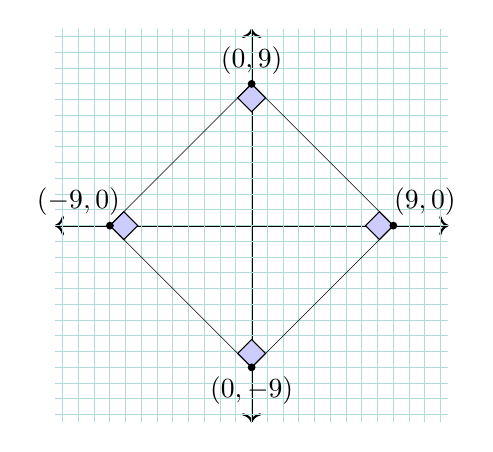
\begin{tikzpicture}
  % axis
  \draw[thick, <->] (0, -2.5) -- (0, 2.5);
  \draw[thick, <->] (-2.5, 0) -- (2.5, 0);

  % grid
  \draw[help lines, step = 0.2cm] (-2.5, -2.5) grid (2.5, 2.5);
  % modified code from https://tex.stackexchange.com/questions/380488/how-can-i-put-a-small-dot
  \tkzDefPoint(0,1.8){B}
\tkzDefPoint(0,-1.8){A}
\tkzDefPoint(1.8,0){C}
\tkzDefPoint(-1.8,0){D}
\tkzLabelPoint[below](A){$(0,-9)$}
\tkzLabelPoint[above](B){$(0,9)$}
\tkzLabelPoint[above,xshift=4mm](C){$(9,0)$}
\tkzLabelPoint[above,xshift=-4mm](D){$(-9,0)$}
\tkzDrawSegment[black!60!black](A,D)
\tkzDrawSegment[black!60!black](B,D)
\tkzDrawSegment[black!60!black](A,C)
\tkzDrawSegment[black!60!black](B,C)
\tkzMarkRightAngle[fill=blue!20,size=0.25](C,A,D)
\tkzMarkRightAngle[fill=blue!20,size=0.25](C,B,D)
\tkzMarkRightAngle[fill=blue!20,size=0.25](A,C,B)
\tkzMarkRightAngle[fill=blue!20,size=0.25](A,D,B)
\foreach \n in {A,B,C,D}
  \node at (\n)[circle,fill,inner sep=1.0pt]{};
\end{tikzpicture}
\subsection{Example Output}
0 2 0 -2 2 0 -2 0
\end{document}
